\documentclass[12pt,a4paper,final]{beamer}
\usetheme{PaloAlto}

\usepackage[utf8]{inputenc}
\usepackage[portuguese]{babel}
\usepackage[T1]{fontenc}
\usepackage{graphicx}

\author{Warley Santos}
\title{Informática Básica Aula 1}
\institute{Associação Gesto de Amor}
\date{2018}
\logo{
\includegraphics[scale=0.058]{imagens/logo.jpg}}

\begin{document}
% Page 1
	\begin{frame}
		\titlepage
	\end{frame}
% Page 2
    \section{O que é informática?}
        \subsection{Concepção}
            \begin{frame}
                \frametitle{O que é Informática?}
                \framesubtitle{Concepção}
                \begin{block}{Origem da palavra:}
                    Em 1956, o cientista da computação alemão \textbf{Karl Steinbuch} publicou o periódico:
                 \end{block}
                 \begin{block}{}
                    \emph{\textbf{Informática:} Processamento Automático de Informação}
                \end{block}
                \begin{block}{}
                     \centering
                     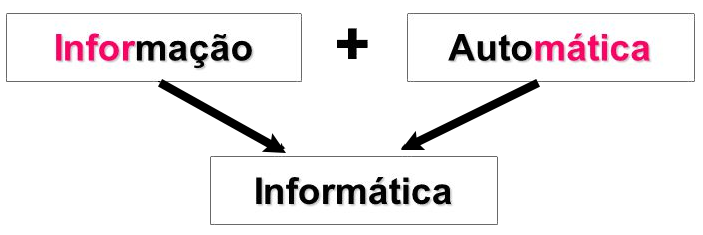
\includegraphics[scale=0.3]{Imagens/informatica.png}
                \end{block}
            \end{frame}
% Page 3
        \subsection{Pirâmide do Conhecimento}
            \begin{frame}
                \frametitle{O que é Informática?}
                \framesubtitle{Pirâmide do Conhecimento}
                    \begin{block}{}
                         \centering
                         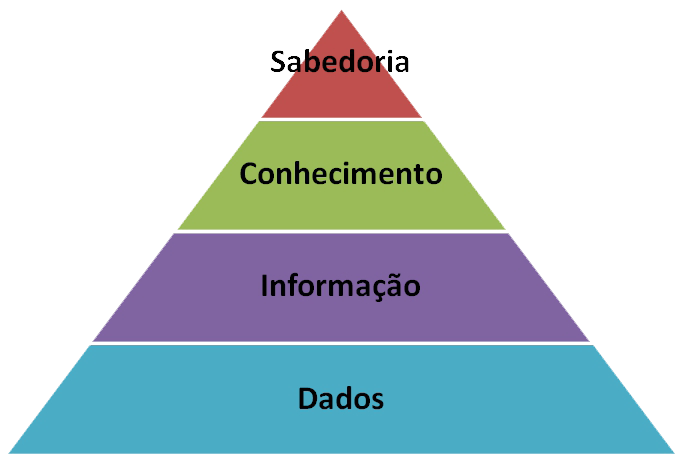
\includegraphics[scale=0.5]{Imagens/piramede.png}
                    \end{block}
	        \end{frame}
% Page 4
    \section{História}
        \subsection{Dígito}
            \begin{frame}
                \frametitle{Um Pouco de história}
                \framesubtitle{Dígito}
                \begin{block}{Nos primórdios:}
                    Primeira maneira que os seres humanos encontraram para expressar quantidade.
                \end{block}
                \begin{block}{}
                    \centering
                    \textcolor{blue}{\large \textbf{Digitus = Dedo, em latim}}
                \end{block}
                \begin{block}{}
                     \centering
                     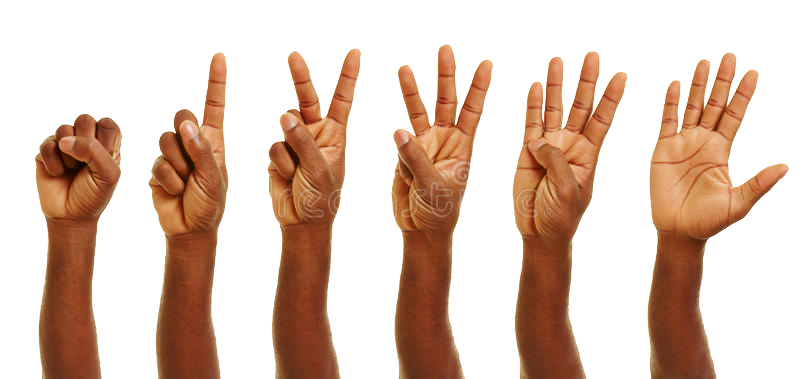
\includegraphics[scale=1]{Imagens/maos.png}
                \end{block}
            \end{frame}
% Page 5
        \subsection{Calculo}
            \begin{frame}
                \frametitle{Um Pouco de história}
                \framesubtitle{Calculo}
                \begin{block}{Nos primórdios:}
                    Empilhamento de pedrinhas para saber a quantidade de ovelhas no rebanho.
                \end{block}
                \begin{block}{}
                    \centering
                    \textcolor{blue}{\large \textbf{Calculus = Pedra, em latim}}
                \end{block}
                \begin{block}{}
                     \centering
                     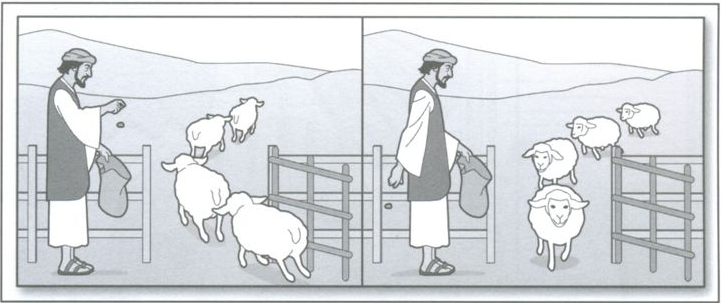
\includegraphics[scale=0.4]{Imagens/ovelhas.png}
                \end{block}
            \end{frame}
% Page 6
        \subsection{Ábaco}
            \begin{frame}
                \frametitle{Um Pouco de história}
                \framesubtitle{Calculo}
                \begin{block}{Nos primórdios:}
                   Foi um dos primeiros instrumentos desenvolvidos para auxiliar os humanos na realização de cálculos. Existem evidências deles na Babilônia no ano 300 A.C.
                \end{block}
                \begin{block}{}
                     \centering
                     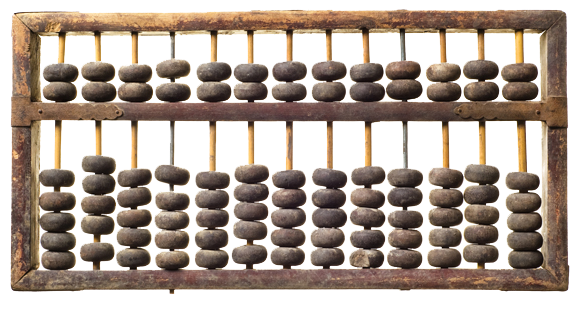
\includegraphics[scale=1.2]{Imagens/abaco.png}
                \end{block}
            \end{frame}

\end{document}
